\documentclass[landscape]{article}

\usepackage[paperwidth=48in,paperheight=36in,margin=1.0in]{geometry}
\usepackage{multicol}
\usepackage{booktabs}
\usepackage{array}
\usepackage{xcolor}
\usepackage{tikz}
\usepackage{helvet}
\renewcommand{\familydefault}{\sfdefault}
\pagestyle{empty}

\definecolor{accent}{RGB}{20,94,130}
\definecolor{soft}{RGB}{235,244,248}
\definecolor{ink}{RGB}{25,30,35}
\definecolor{warn}{RGB}{137,76,30}

\newcommand{\blocktitle}[1]{\vspace{0.22in}\noindent{\color{accent}\Huge\bfseries #1}\par\vspace{0.10in}}
\newcommand{\posterbox}[1]{%
  \vspace{0.12in}
  \noindent\colorbox{soft}{%
    \begin{minipage}{0.96\linewidth}
    \vspace{0.15in}
    #1
    \vspace{0.15in}
    \end{minipage}}
  \vspace{0.12in}
}

\begin{document}
\color{ink}

\begin{center}
{\fontsize{56}{62}\selectfont\bfseries Middle-Model Verification for Three-Tier Speculative Decoding}\\[0.15in]
{\fontsize{32}{38}\selectfont A Systems Evaluation on Reasoning-Oriented Generation}\\[0.12in]
{\LARGE Zichu Wu \quad Gaokai Zhang \quad Melody Yin}\\[0.06in]
{\Large MLSys Course Project, April 2026}
\end{center}

\vspace{0.18in}

\posterbox{
{\Huge\bfseries Main takeaway.}
{\Huge A middle verifier can improve reasoning quality, but it is not a free speedup. On GSM8K, selective three-tier decoding improves exact match from 0.3541 to 0.3753; on MMLU, accuracy is effectively unchanged, so the middle tier mostly adds overhead.}
}

\begin{multicols}{3}

\blocktitle{Question}

Speculative decoding lets a small model draft candidate tokens and a large model verify them. We ask whether a third, intermediate model can make this pipeline more useful:

\vspace{0.08in}
\begin{center}
{\LARGE Small drafter $\rightarrow$ Middle verifier $\rightarrow$ Large verifier}
\end{center}

The hypothesis is task-dependent. The middle model is useful only if filtering weak drafts improves final answers or saves enough large-model work to offset its own verification cost.

\begin{center}
\begin{tabular}{lll}
\toprule
Tier & Model & Role \\
\midrule
Small & Qwen2.5-0.5B & draft tokens \\
Middle & Qwen2.5-1.5B & filter and route \\
Large & Qwen2.5-14B & final verification \\
\bottomrule
\end{tabular}
\end{center}

\blocktitle{Method}

The fixed-window hierarchy verifies short small-model drafts with the middle model, accumulates accepted middle tokens, and sends the resulting block to the large model.

\begin{center}
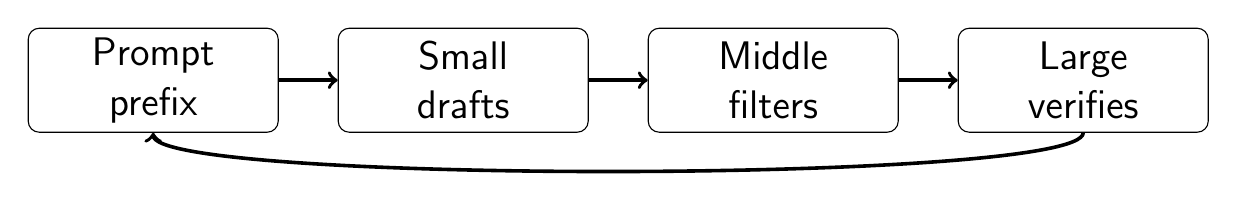
\begin{tikzpicture}[node distance=1.55in, every node/.style={draw, rounded corners, align=center, minimum width=1.25in, minimum height=0.52in, font=\Large}]
\node (p) {Prompt\\prefix};
\node[right of=p] (s) {Small\\drafts};
\node[right of=s] (m) {Middle\\filters};
\node[right of=m] (l) {Large\\verifies};
\draw[->, line width=1.3pt] (p) -- (s);
\draw[->, line width=1.3pt] (s) -- (m);
\draw[->, line width=1.3pt] (m) -- (l);
\draw[->, line width=1.3pt] (l.south) .. controls +(0,-0.65) and +(0,-0.65) .. (p.south);
\end{tikzpicture}
\end{center}

Final configurations:
\begin{itemize}
\item \texttt{baseline\_sw5}: tuned two-layer baseline.
\item \texttt{fixed\_cascade}: always route through the middle verifier.
\item \texttt{adaptive}: update draft windows using recent utility.
\item \texttt{selective}: use recent utility to decide whether to call the middle model.
\item \texttt{cost-aware}: bypass the middle when measured utility or acceptance is too low.
\end{itemize}

\blocktitle{GSM8K Result}

Full 1319-sample focused comparison against the tuned two-layer baseline:

\begin{center}
\begin{tabular}{lrrr}
\toprule
Method & Tok/s & Score & $\Delta$ score \\
\midrule
\texttt{baseline\_sw5} & 33.716 & 0.3541 & 0.0000 \\
\texttt{fixed\_cascade} & 30.993 & 0.3874 & +0.0334 \\
\texttt{adaptive} & 31.881 & 0.3723 & +0.0182 \\
\texttt{selective} & 32.347 & 0.3753 & +0.0212 \\
\texttt{cost-aware} & 31.331 & 0.3541 & 0.0000 \\
\bottomrule
\end{tabular}
\end{center}

\posterbox{
{\LARGE GSM8K is the positive result. Fixed, adaptive, and selective middle verification improve exact match; selective routing gives the best completed speed-quality compromise among methods that improve score.}
}

\blocktitle{Cost-Aware Routing}

Cost-aware routing is useful as a diagnostic, but this setting was too conservative on GSM8K.

\begin{center}
\begin{tabular}{lrrr}
\toprule
Dataset & Method & Middle route & Score \\
\midrule
GSM8K & \texttt{selective} & 93.6\% & 0.3753 \\
GSM8K & \texttt{cost-aware} & 3.3\% & 0.3541 \\
MMLU & \texttt{selective} & 92.9\% & 0.3257 \\
MMLU & \texttt{cost-aware} & 7.5\% & 0.3242 \\
\bottomrule
\end{tabular}
\end{center}

The policy can remove middle-model calls, but if it bypasses the middle verifier too often it also removes the quality gain.

\blocktitle{MMLU Boundary Result}

Full 14,042-sample MMLU focused comparison:

\begin{center}
\begin{tabular}{lrrr}
\toprule
Method & Tok/s & Accuracy & $\Delta$ acc. \\
\midrule
\texttt{baseline\_sw5} & 24.864 & 0.3243 & 0.0000 \\
\texttt{fixed\_cascade} & 18.692 & 0.3256 & +0.0013 \\
\texttt{adaptive} & 19.655 & 0.3255 & +0.0011 \\
\texttt{selective} & 19.946 & 0.3257 & +0.0014 \\
\texttt{cost-aware} & 23.552 & 0.3242 & -0.0001 \\
\bottomrule
\end{tabular}
\end{center}

MMLU is short and multiple-choice, so there is little generation trajectory for the middle verifier to repair. Cost-aware routing recovers much of the throughput loss but does not improve accuracy.

\posterbox{
{\color{warn}\LARGE Throughput caveat.} {\LARGE One final MMLU shard was repaired on Modal A100 with all models on one GPU, while the original shards used two L40S GPUs. Accuracy is full-dataset; MMLU throughput should be read with this mixed-hardware caveat.}
}

\blocktitle{Why It Happens}

The middle layer helps only when:

\begin{center}
{\LARGE large-model benefit $>$ middle-model cost}
\end{center}

GSM8K has long reasoning traces, so filtering early weak continuations can change the final answer. MMLU answers are short and constrained, so middle verification often adds cost without changing the prediction.

\blocktitle{System Work}

\begin{center}
\begin{tabular}{p{0.34\linewidth}p{0.52\linewidth}}
\toprule
Component & Contribution \\
\midrule
Scoring layer & Extracted GSM8K numeric answers and MMLU choices. \\
ACSD prototype & Tested middle pre-verification and proxy stopping. \\
Fixed-window harness & Main Qwen 0.5B $\rightarrow$ 1.5B $\rightarrow$ 14B benchmark. \\
Routing policies & Adaptive, selective, and cost-aware middle routing. \\
Reliability & Strict shard validation, repair jobs, and Modal subshards. \\
\bottomrule
\end{tabular}
\end{center}

\blocktitle{Conclusion}

{\LARGE Three-tier speculative decoding should be treated as a routing policy, not as an automatic speedup. The middle verifier is useful as a quality filter on reasoning-heavy generation, but it must be called selectively and calibrated carefully.}

\vfill
{\large References: Leviathan et al., \emph{Fast Inference from Transformers via Speculative Decoding}; Chen et al., \emph{Speculative Sampling}; Cascade Speculative Drafting.}

\end{multicols}
\end{document}
